\documentclass[conference]{IEEEtran}

% IEEE ICIT 2027 - preliminary manuscript based on the available experimental text.
% Regular papers: up to 6 pages (including references).
% IMPORTANT: Review every TODO before submission. No missing results have been invented.
% Figures are generated by scripts/make_figures.py from
% pid_serial_tuner/lqr_tuner/data/coleta_lqr_20261025_004214.csv.
\usepackage{cite}
\usepackage{amsmath,amssymb,amsfonts}
\usepackage{graphicx}
\usepackage{booktabs}
\usepackage{array}
\usepackage{tikz}
\usetikzlibrary{arrows.meta,positioning}
\graphicspath{{figures/}}

\begin{document}

\title{Adaptive Fuzzy Microstepping for Disturbance Rejection in a Stepper-Driven Furuta Pendulum}

% Three author columns with names kept on a single line.
% Academic titles are included as requested; verify conference indexing rules before submission.
\author{%
\begin{minipage}[t]{0.26\textwidth}\centering
{\small\bfseries\mbox{Jos\'{e} Anderson da Silva}\par}
{\footnotesize
\textit{Universidade Federal de Alagoas (UFAL)}\par
Macei\'{o}, Brazil\par
jandersons@ic.ufal.br\par}
\end{minipage}\hfill
\begin{minipage}[t]{0.32\textwidth}\centering
{\small\bfseries\mbox{Prof. Dr. Tiago Alves de Almeida}\par}
{\footnotesize
\textit{Universidade Federal de Alagoas (UFAL)}\par
Macei\'{o}, Brazil\par
tiagoalves@ic.ufal.br\par}
\end{minipage}\hfill
\begin{minipage}[t]{0.40\textwidth}\centering
{\small\bfseries\mbox{Prof. Dr. \'{I}caro Bezerra Queiroz de Ara\'{u}jo}\par}
{\footnotesize
\textit{Universidade Federal de Alagoas (UFAL)}\par
Macei\'{o}, Brazil\par
icaro@ic.ufal.br\par}
\end{minipage}%
}

\maketitle

\begin{abstract}
This paper investigates adaptive microstepping for a stepper-driven Furuta pendulum, aiming to reconcile smooth motion during nominal stabilization with recovery from external disturbances. The experimental platform employs a discrete-time linear quadratic regulator (LQR) and a reduced-order state observer, while a fuzzy supervisor adjusts the motor microstepping resolution according to pendulum angular deviation and estimated angular velocity. A zero-order Sugeno rule base selects among five microstepping resolutions, from 1/16 to 1/256. Because the step-pulse rate is bounded, each resolution imposes a ceiling on the commanded arm velocity, which is lowest for the finest subdivision. In a single experimental session comparing the adaptive scheme with five fixed resolutions, the fixed 1/256 and 1/128 configurations lost balance after impulsive disturbances once the velocity command saturated at that ceiling, whereas fixed 1/32 and 1/16 operation retained balance during nominal operation but increased the steady-state RMS pendulum deviation from $0.16^\circ$ (1/256) to $0.39^\circ$ and $0.79^\circ$, respectively. The adaptive configuration recovered from both applied disturbances while keeping a steady-state RMS deviation of $0.17^\circ$. These results are preliminary; repeated trials with controlled disturbance magnitude are still required to quantify the trade-off statistically.
\end{abstract}

\begin{IEEEkeywords}
Furuta pendulum, stepper motor, microstepping, fuzzy supervisor, disturbance rejection, motion control.
\end{IEEEkeywords}

\section{Introduction}
Rotary inverted pendulums are widely used to investigate feedback stabilization, state estimation, and disturbance rejection in underactuated mechatronic systems \cite{akhtaruzzaman2010}. In a stepper-driven implementation, closed-loop behavior depends not only on the control algorithm but also on the interface that converts the controller output into motor excitation.

Microstepping subdivides a full step into smaller increments of the commanded winding-current profile. Fine resolutions can improve motion smoothness, although the available incremental torque for each individual microstep decreases as the subdivision becomes finer \cite{ti2021}. This does not mean that the motor's maximum holding torque increases when a coarser resolution is selected. Instead, the effective behavior depends on the motor, current regulation, loading, pulse timing, and mechanical transmission.

In the prototype considered here, fixed 1/256 microstepping provides comparatively smooth motion near the upright equilibrium. Coarser operation, such as 1/32 or 1/16, can maintain balance but produces more abrupt movements of the rotary arm and larger oscillations of the pendulum. Conversely, high-resolution fixed operation has presented difficulty in recovering from externally applied disturbances. These observations describe the investigated plant; they are not assumed to hold universally for every stepper drive.

The central hypothesis of this study is that \emph{adapting microstepping resolution to the pendulum's instantaneous motion can preserve fine control near equilibrium while improving the response during large deviations}. Rather than modifying the stabilizing controller, the proposed approach places a fuzzy supervisor at the actuator interface.

The intended contributions are: (i) a state-dependent microstepping supervisor with five discrete drive resolutions; (ii) its integration with a fixed discrete LQR and reduced-order observer; and (iii) an experimental comparison against five fixed resolutions that assesses both nominal smoothness and recovery from disturbances, and that relates recovery failures to the velocity ceiling imposed by each resolution. Preliminary evidence is reported without claiming statistical superiority.

% TODO (literature): Add and contrast papers directly related to adaptive
% microstepping, switching stepper drive modes, and fuzzy drive supervision.

\section{Experimental Platform and Control Architecture}
\subsection{Physical platform and sensing}
The experimental platform is a rotary inverted pendulum comprising a horizontal arm driven by a stepper motor and a pendulum free to rotate in a vertical plane. The arm angle is denoted by $\theta$ and the pendulum angle relative to the unstable upright position by $\alpha$. Both angles are measured by 12-bit AS5600 magnetic angle sensors, which yields a resolution of $360^\circ/4096\approx0.088^\circ$. The controller is executed on an embedded microcontroller with sampling period $T_s=2\,\mathrm{ms}$.

The previously documented dimensions are $r=0.12495\,\mathrm{m}$ for the rotating arm and $L=0.2043271\,\mathrm{m}$ for the pendulum length parameter employed in the linearized model. These parameters describe the present prototype and are not a general requirement of the proposed supervisor.

% TODO (hardware): Name the actual microcontroller, stepper motor, driver,
% electrical current limit, supply voltage, transmission ratio,
% and mechanical loading.

\subsection{Baseline state-feedback controller}
The stabilizer is a discrete-time LQR designed around the upright equilibrium. The state vector and commanded arm acceleration are
\begin{equation}
 x_k = [\theta_k,\alpha_k,\dot\theta_k,\dot\alpha_k]^T,\qquad
 u_k=\ddot\theta_{\mathrm{cmd},k}.
 \label{eq:state}
\end{equation}
Because only angular positions are directly measured, a reduced-order observer estimates $\dot\theta$ and $\dot\alpha$. The LQR command is
\begin{equation}
 u_k=-K_d\begin{bmatrix}
 \theta_k & \alpha_k & \hat{\dot\theta}_k & \hat{\dot\alpha}_k
 \end{bmatrix}^{T}.
 \label{eq:lqr}
\end{equation}
For the reported experimental design, the nominal LQR weights and calculated gain are
\begin{equation}
 Q=\operatorname{diag}(2500,3000,500,20),\qquad R=2,
\end{equation}
\begin{equation}
 K_d=\begin{bmatrix}-34.3113 & 763.3819 & -28.8791 & 127.0982\end{bmatrix}.
 \label{eq:gain}
\end{equation}
% TODO (check): the firmware log of 25 Oct. 2026 reports
% K_d = [-34.311304, 763.316351, -28.879132, 127.087297]; confirm which gain is final.
Both the observer and the LQR are kept unchanged when comparing the actuator operating modes. The acceleration reference is integrated into an angular velocity command,
\begin{equation}
 \omega_{\mathrm{cmd},k}=\omega_{\mathrm{cmd},k-1}+u_k T_s,
 \label{eq:int}
\end{equation}
which is converted into a step-pulse frequency:
\begin{equation}
 f_{\mathrm{step},k}=\frac{|\omega_{\mathrm{cmd},k}|}{2\pi}
 N_{\mathrm{steps}}\,\mu_k\,G.
 \label{eq:pulse}
\end{equation}
Here, $N_{\mathrm{steps}}$ is the number of full motor steps per revolution, $\mu_k$ denotes microsteps per full step, and $G$ represents the mechanical transmission ratio, when present. Equation~\eqref{eq:pulse} makes explicit that the commanded pulse rate must be recalculated when microstepping resolution changes so that the nominal angular velocity reference remains consistent.

The pulse generator is bounded by $f_{\max}=23\,\mathrm{kHz}$, a value determined experimentally on the test bench. Inverting \eqref{eq:pulse}, each resolution therefore admits a maximum commanded velocity
\begin{equation}
 \omega_{\max}(\mu)=\frac{2\pi f_{\max}}{N_{\mathrm{steps}}\,\mu\,G},
 \label{eq:wmax}
\end{equation}
beyond which $\omega_{\mathrm{cmd}}$ is saturated. With $N_{\mathrm{steps}}=200$ and $G=1$, $\omega_{\max}$ equals $2.82$, $5.65$, $11.3$, $22.6$, and $45.2\,\mathrm{rad/s}$ for $\mu=256$, $128$, $64$, $32$, and $16$, respectively. Fine subdivisions thus restrict the arm velocity available to counteract a disturbance, which is the limitation the proposed supervisor addresses.
% TODO (check): confirm G = 1 (direct drive) for the final hardware description.

% TODO (critical implementation): Explain how driver microstep-mode switching
% preserves the phase/current reference and positional continuity, and report
% any limitations or transients caused by switching. A pulse-rate rescaling
% alone does not guarantee a transient-free physical transition.

\begin{figure*}[t]
\centering
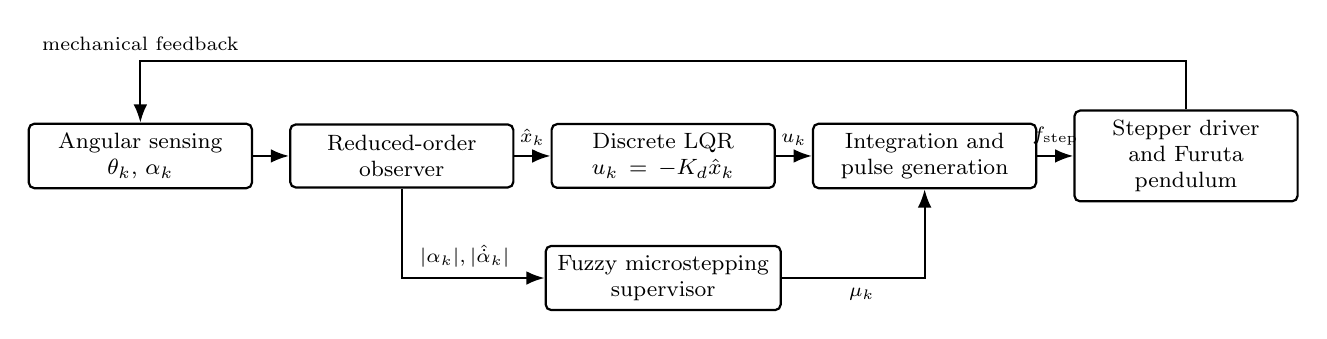
\begin{tikzpicture}[
 >=Latex, thick,
 block/.style={draw,rounded corners=2pt,align=center,font=\footnotesize,
              minimum height=0.80cm,text width=2.60cm},
 smallblock/.style={draw,rounded corners=2pt,align=center,font=\footnotesize,
              minimum height=0.75cm,text width=2.75cm}
]
 \node[block] (sensor) at (0,0) {Angular sensing\\$\theta_k$, $\alpha_k$};
 \node[block] (observer) at (3.32,0) {Reduced-order\\observer};
 \node[block] (lqr) at (6.64,0) {Discrete LQR\\$u_k=-K_d\hat x_k$};
 \node[block] (pulse) at (9.96,0) {Integration and\\pulse generation};
 \node[block] (plant) at (13.28,0) {Stepper driver\\and Furuta pendulum};
 \draw[->] (sensor) -- (observer);
 \draw[->] (observer) -- node[above,font=\scriptsize] {$\hat x_k$} (lqr);
 \draw[->] (lqr) -- node[above,font=\scriptsize] {$u_k$} (pulse);
 \draw[->] (pulse) -- node[above,font=\scriptsize] {$f_{\rm step}$} (plant);
 \node[smallblock] (fuzzy) at (6.64,-1.55) {Fuzzy microstepping\\supervisor};
 \draw[->] (observer.south) |- node[pos=0.72,above,font=\scriptsize] {$|\alpha_k|,|\hat{\dot\alpha}_k|$} (fuzzy.west);
 \draw[->] (fuzzy.east) -| node[pos=0.28,below,font=\scriptsize] {$\mu_k$} (pulse.south);
 \draw[->] (plant.north) -- ++(0,0.62) -| node[pos=0.5,above,font=\scriptsize] {mechanical feedback} (sensor.north);
\end{tikzpicture}
\caption{Control architecture: the LQR and observer remain unchanged, while the fuzzy supervisor modifies the microstepping setting used by pulse generation.}
\label{fig:architecture}
\end{figure*}

\section{Proposed Fuzzy Microstepping Supervisor}
\subsection{Design principle and variables}
The fuzzy supervisor is an auxiliary layer for selecting the stepper-drive resolution. It does not replace the LQR stabilization law. The inputs are the magnitude of the pendulum angular deviation and estimated angular velocity:
\begin{equation}
 e_{\alpha,k}=|\alpha_k|,\qquad e_{\dot\alpha,k}=|\hat{\dot\alpha}_k|.
 \label{eq:inputs}
\end{equation}
The output is restricted to the five microstepping settings used in the proposed implementation:
\begin{equation}
 \mu_k\in\mathcal M=\{16,32,64,128,256\}.
 \label{eq:modes}
\end{equation}
A value $\mu=256$ denotes 1/256 full-step operation, and $\mu=16$ denotes 1/16 full-step operation. The highest subdivision is preferred for small motion around the equilibrium; coarser subdivisions are selected in more demanding recovery conditions.

\subsection{Membership functions and inference}
A zero-order Sugeno fuzzy inference structure is employed. Each input uses three trapezoidal linguistic sets. For the angular deviation, over the design interval $e_\alpha\in[0,6]^\circ$, the sets are defined as
\begin{align}
 \mathrm{Small}:&(0,0,2,3),\nonumber\\
 \mathrm{Medium}:&(2,3,4,5),\\
 \mathrm{Large}:&(4,5,6,6),\nonumber
\end{align}
where the four entries represent the trapezoid breakpoints $(a,b,c,d)$ in degrees. For angular velocity, over $e_{\dot\alpha}\in[0,150]^\circ/\mathrm{s}$, the definitions are
\begin{align}
 \mathrm{Low}:&(0,0,15,40),\nonumber\\
 \mathrm{Medium}:&(25,50,70,95),\\
 \mathrm{High}:&(80,110,150,150).\nonumber
\end{align}
The breakpoints and inference universes are those reported in the existing implementation description. Handling of inputs outside these intervals should be explicitly checked in firmware.

The nine rules are summarized in Table~\ref{tab:rules}. Each rule $i$ has a constant consequent $\mu_i\in\mathcal M$. If $w_i$ denotes its firing strength, the aggregated output is
\begin{equation}
 \widetilde\mu_k = \frac{\sum_{i=1}^{9}w_i\mu_i}{\sum_{i=1}^{9}w_i},\qquad
 \mu_k=\mathcal Q_{\mathcal M}(\widetilde\mu_k),
 \label{eq:sugeno}
\end{equation}
where $\mathcal Q_{\mathcal M}$ selects the closest supported microstepping level. The precise conjunction operator and tie-breaking procedure must match the embedded code.

\begin{table}[t]
\caption{Rule base of the fuzzy microstepping supervisor}
\label{tab:rules}
\centering\footnotesize
\begin{tabular}{ccc}
\toprule
$|\alpha|$ & $|\hat{\dot\alpha}|$ & Microsteps/full step\\
\midrule
Small & Low & 256\\
Small & Medium & 128\\
Small & High & 64\\
Medium & Low & 128\\
Medium & Medium & 64\\
Medium & High & 32\\
Large & Low & 16\\
Large & Medium & 16\\
Large & High & 16\\
\bottomrule
\end{tabular}
\end{table}

\subsection{Temporary switching and rearming}
The reported strategy also employs timing logic to avoid excessive switching between adjacent microstepping modes. Upon disturbance detection, a lower-resolution configuration is retained during a recovery period $T_{\mathrm{hold}}$. Afterwards, the system returns toward higher resolution. New disturbance detection is inhibited for an additional interval $T_{\mathrm{block}}$ and reenabled only after a predefined stable condition is reached. This limits repeated switching while the pendulum crosses the nominal operating region.

This scheduling logic is separate from the fuzzy rule base and should be reproduced in sufficient detail to allow experimental replication. The microstepping transitions must be implemented in accordance with the selected driver's mode-switching behavior.

% TODO (supervisor): Fill in actual values of T_hold, T_block, stable region,
% trigger/rearm rules, fuzzy AND operator, update rate, and numerical handling
% of values beyond the membership-function design ranges.
% Firmware defaults (config.h): LQR_DISTURBANCE_HOLD_MS = 1000,
% LQR_DISTURBANCE_REARM_BLOCK_MS = 1200, LQR_DISTURBANCE_REARM_STABLE_MS = 350,
% rearm when |alpha| < 1 deg and |alpha_dot| < 20 deg/s. In the 25 Oct. 2026
% session the descent ramp used 100 ms per level (see Fig. 4, bottom panel).

\section{Experimental Evaluation Methodology}
Six drive configurations were evaluated with the same LQR and observer gains: the proposed fuzzy adaptive microstepping and fixed resolutions of 1/256, 1/128, 1/64, 1/32, and 1/16. All configurations were recorded in a single session, each after its own swing-up and capture, and telemetry ($\alpha$, $\theta$, $u$, $\omega_{\mathrm{cmd}}$, and the active $\mu$) was logged at $50\,\mathrm{Hz}$.

\subsection{Nominal stabilization and smoothness}
For each mode, an $8\,\mathrm{s}$ interval without deliberate disturbances was selected, excluding the swing-up and capture transient and the recovery following any disturbance. Nominal angular regulation is evaluated through
\begin{equation}
 \alpha_{\mathrm{RMS}}=\sqrt{\frac{1}{N}\sum_{k=1}^{N}\alpha_k^2},
 \label{eq:rms}
\end{equation}
complemented by the 95th percentile of $|\alpha|$, the standard deviation $\sigma_\theta$ of the arm angle about its local mean, and the RMS value of the control command $u$. These measures characterize the abrupt arm movements associated with coarse fixed microstepping and are computed over identical window durations for every mode.

\subsection{Disturbance recovery}
Impulsive disturbances were applied manually to the pendulum while it was stabilized. Because their magnitude was not controlled, the peak pendulum angular rate within the first $80\,\mathrm{ms}$ after impact, $|\dot\alpha|_0$, obtained by finite differences, is reported as a proxy for disturbance intensity. A trial is classified as a loss of balance when $|\alpha|$ exceeds $20^\circ$, the threshold at which the firmware disengages the LQR. For each impact, the peak $|\alpha|$, the peak $|\omega_{\mathrm{cmd}}|$, and the commanded microstepping trajectory $\mu(t)$ are recorded alongside $\alpha(t)$ and $\theta(t)$. With repeated trials, the recovery fraction
\begin{equation}
 P_{\mathrm{rec}}=100\,\frac{N_{\mathrm{recovered}}}{N_{\mathrm{trials}}}\%
 \label{eq:success}
\end{equation}
can be estimated for each mode.

% TODO (experiments): Describe the tool used to apply the impacts; select a
% repeatable disturbance method with measured magnitude; define the recovery
% tolerance band and time-to-recover; increase the number of trials per mode.

\section{Experimental Results and Discussion}

\begin{figure*}[t]
\centering
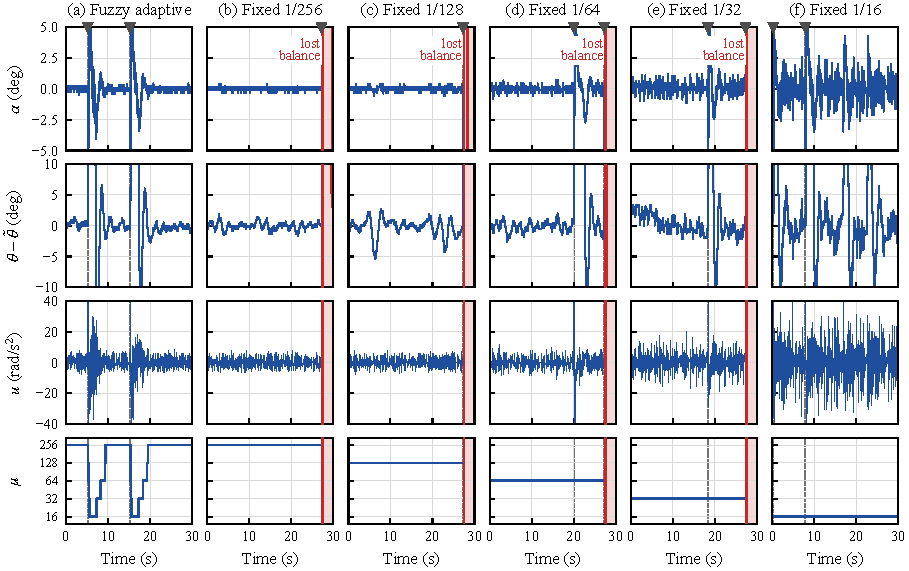
\includegraphics[width=\textwidth]{fig_last30s.pdf}
\caption{Last $30\,\mathrm{s}$ of stabilization for each drive configuration: pendulum angle $\alpha$, arm angle about its window median $\theta-\tilde\theta$, LQR command $u$, and active microstepping setting $\mu$. All columns share the same vertical scales, which are limited to resolve the steady-state behavior; excursions during impacts exceed the plotted range (full-scale responses in Fig.~\ref{fig:disturbance}). Triangles and dashed lines mark impacts; the red line and shaded region mark loss of balance, after which the LQR is disengaged.}
\label{fig:steady}
\end{figure*}

\begin{table}[t]
\caption{Nominal stabilization metrics over disturbance-free $8\,\mathrm{s}$ windows}
\label{tab:steady}
\centering\footnotesize
\setlength{\tabcolsep}{4pt}
\begin{tabular}{lcccc}
\toprule
Mode & $\alpha_{\mathrm{RMS}}$ ($^\circ$) & $|\alpha|_{95}$ ($^\circ$) & $\sigma_\theta$ ($^\circ$) & $u_{\mathrm{RMS}}$ (rad/s$^2$)\\
\midrule
Fuzzy adaptive & 0.17 & 0.33 & 0.45 & 2.43\\
Fixed 1/256 & 0.16 & 0.34 & 0.49 & 2.35\\
Fixed 1/128 & 0.18 & 0.39 & 1.98 & 2.05\\
Fixed 1/64 & 0.22 & 0.45 & 0.86 & 2.78\\
Fixed 1/32 & 0.39 & 0.76 & 0.93 & 4.36\\
Fixed 1/16 & 0.79 & 1.70 & 2.26 & 10.22\\
\bottomrule
\end{tabular}
\end{table}

\subsection{Nominal stabilization}
Fig.~\ref{fig:steady} summarizes the last $30\,\mathrm{s}$ of each configuration, including the applied impacts, and Table~\ref{tab:steady} quantifies the regulation over disturbance-free $8\,\mathrm{s}$ windows taken from the same recordings. Every configuration sustained the upright equilibrium in the absence of deliberate disturbances, but with markedly different regulation quality. Fixed 1/256 operation kept $\alpha$ within approximately $\pm0.4^\circ$, close to the $0.088^\circ$ quantization of the angle sensor. As the subdivision became coarser, the pendulum deviation and the control activity grew monotonically from 1/128 onward: relative to 1/256, $\alpha_{\mathrm{RMS}}$ increased by factors of $2.4$ and $4.9$, and $u_{\mathrm{RMS}}$ by factors of $1.9$ and $4.3$, for 1/32 and 1/16, respectively. The arm motion under 1/16 operation also exhibited abrupt excursions of up to about $6^\circ$. Hence, coarse fixed microstepping keeps the pendulum balanced but cannot reproduce the fine regulation obtained with 1/256. The arm-angle deviation under 1/128 was dominated by a single slow excursion within the window, which explains its comparatively large $\sigma_\theta$.

The adaptive configuration remained at $\mu=256$ during nominal operation, and its metrics were practically indistinguishable from those of fixed 1/256 operation ($\alpha_{\mathrm{RMS}}=0.17^\circ$ versus $0.16^\circ$). Fig.~\ref{fig:steady} also contrasts the two extremes of the trade-off: fixed 1/256 and 1/128 operation lost balance at their first impact, whereas fixed 1/16 operation withstood both of its impacts while exhibiting the largest steady-state oscillations. In this session, only the adaptive configuration combined fine regulation with recovery, reducing $\mu$ during each impact and returning to $\mu=256$ afterwards.

\begin{figure}[t]
\centering
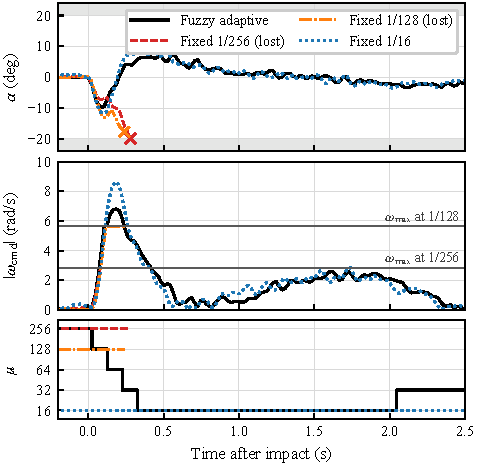
\includegraphics[width=\columnwidth]{fig_disturbance.pdf}
\caption{Representative responses to impulsive disturbances, aligned at the impact instant: pendulum angle (top), commanded arm velocity with the ceilings $\omega_{\max}$ of \eqref{eq:wmax} for 1/256 and 1/128 (middle), and active microstepping setting (bottom). Shaded bands mark $|\alpha|>20^\circ$, where the LQR is disengaged; crosses mark loss of balance.}
\label{fig:disturbance}
\end{figure}

\begin{table}[t]
\caption{Response to each applied disturbance}
\label{tab:impacts}
\centering\footnotesize
\setlength{\tabcolsep}{3.5pt}
\begin{tabular}{lccccc}
\toprule
Mode & $|\dot\alpha|_0$ ($^\circ$/s) & Peak $|\alpha|$ ($^\circ$) & Peak $|\omega_{\mathrm{cmd}}|$ & $\omega_{\max}$ & Outcome\\
 & & & (rad/s) & (rad/s) & \\
\midrule
Fuzzy adaptive & 154 & 9.5 & 6.52 & 45.2$^{a}$ & Recovered\\
Fuzzy adaptive & 200 & 9.9 & 6.80 & 45.2$^{a}$ & Recovered\\
Fixed 1/256 & 128 & $>20$ & 2.82 & 2.82 & Lost\\
Fixed 1/128 & 192 & $>20$ & 5.65 & 5.65 & Lost\\
Fixed 1/64 & 202 & 13.6 & 10.28 & 11.3 & Recovered\\
Fixed 1/64 & 212 & $>20$ & 10.81 & 11.3 & Lost\\
Fixed 1/32 & 97 & 5.5 & 4.65 & 22.6 & Recovered\\
Fixed 1/32 & 216 & $>20$ & 14.94 & 22.6 & Lost\\
Fixed 1/16 & 92 & 7.0 & 4.20 & 45.2 & Recovered\\
Fixed 1/16 & 193 & 11.8 & 8.66 & 45.2 & Recovered\\
\bottomrule
\multicolumn{6}{l}{\scriptsize $^{a}$Ceiling at the coarsest level reached, $\mu=16$.}
\end{tabular}
\end{table}

\begin{figure}[t]
\centering
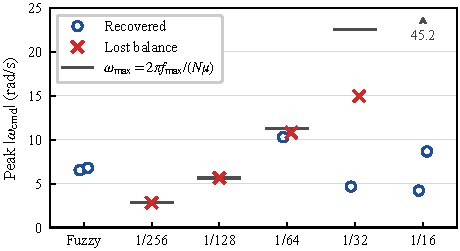
\includegraphics[width=\columnwidth]{fig_speed_ceiling.pdf}
\caption{Peak commanded arm velocity reached after each disturbance (Table~\ref{tab:impacts}) compared with the velocity ceiling of each fixed resolution. The ceiling for 1/16 lies above the vertical range.}
\label{fig:ceiling}
\end{figure}

\subsection{Disturbance recovery}
Table~\ref{tab:impacts} lists the ten impacts identified in the session, and Fig.~\ref{fig:disturbance} superimposes representative responses. Under fixed 1/256 and 1/128 operation, the LQR demanded an arm velocity larger than the corresponding ceiling, so $\omega_{\mathrm{cmd}}$ saturated at $2.82$ and $5.65\,\mathrm{rad/s}$, respectively; the arm could not move fast enough to bring the pendulum back, and $|\alpha|$ exceeded $20^\circ$ within about $0.3\,\mathrm{s}$. The fixed 1/256 configuration fell after an impact with $|\dot\alpha|_0=128^\circ/\mathrm{s}$, the mildest of all disturbances that caused a loss of balance.

The adaptive supervisor reduced the resolution from 1/256 to 1/16 within approximately $0.35\,\mathrm{s}$ of each impact (Fig.~\ref{fig:disturbance}, bottom), stepping through the intermediate levels. The corresponding increase in $\omega_{\max}$ allowed the command to reach $6.5$--$6.8\,\mathrm{rad/s}$, above the 1/256 and 1/128 ceilings, and the pendulum recovered from impacts with $|\dot\alpha|_0$ of $154$ and $200^\circ/\mathrm{s}$, with peak deviations below $10^\circ$. The resolution was subsequently raised again, and the next nominal interval was regulated at $\mu=256$ (Fig.~\ref{fig:steady}a). Its recovery trajectory closely matches that of fixed 1/16 operation under a comparable impact ($193^\circ/\mathrm{s}$), without inheriting the steady-state degradation of 1/16 shown in Table~\ref{tab:steady}.

Fig.~\ref{fig:ceiling} indicates that the velocity ceiling explains the failures of the two finest fixed resolutions and plausibly that of 1/64, whose losing impact drove $\omega_{\mathrm{cmd}}$ to within $5\%$ of its $11.3\,\mathrm{rad/s}$ ceiling. It does not explain the loss under fixed 1/32: there, the most intense impact of the session ($216^\circ/\mathrm{s}$) caused a loss of balance at $14.9\,\mathrm{rad/s}$, well below the $22.6\,\mathrm{rad/s}$ ceiling. Other factors, such as the reduced positional resolution of coarse microstepping or the torque available at high step rates, may therefore also contribute.

\subsection{Limitations}
These results come from a single session with one or two manually applied impacts per mode. The impact intensities were not matched across modes; as Table~\ref{tab:impacts} shows, they ranged from $92$ to $216^\circ/\mathrm{s}$. In particular, no fixed coarse mode was subjected to an impact identical to those recovered by the adaptive configuration. The results thus illustrate the mechanism and motivate the approach, but they do not establish a statistically reproducible improvement. A threshold-based (non-fuzzy) switching baseline would further help determine whether the fuzzy inference provides benefits beyond simpler microstep-mode switching.

\section{Conclusion}
An adaptive microstepping approach has been formulated for a stepper-driven Furuta pendulum using a fuzzy supervisory layer around a fixed discrete-time LQR and reduced-order observer. The supervisor selects among five microstepping resolutions based on the magnitude of the pendulum's angular deviation and estimated angular velocity, favoring fine subdivisions near equilibrium and coarser subdivisions during recovery. Experiments comparing the adaptive scheme with five fixed resolutions showed that coarse fixed microstepping (1/32 and 1/16) maintains balance at the cost of a $2.4$-fold to $4.9$-fold increase in steady-state RMS pendulum deviation, while fine fixed microstepping (1/256 and 1/128) loses balance after disturbances once the commanded arm velocity saturates at the ceiling imposed by the bounded pulse rate. The adaptive configuration matched the steady-state regulation of fixed 1/256 operation and recovered from both applied disturbances. Future work will quantify this trade-off with repeated, magnitude-controlled disturbance trials and compare the fuzzy supervisor with a threshold-based switching baseline.

% TODO (before submission): check the paper fits at most six pages including
% references, verify final PDF size <= 2 MB, and remove all template/provisional comments.

\begin{thebibliography}{00}
\bibitem{akhtaruzzaman2010}
M. Akhtaruzzaman and A. A. Shafie, ``Modeling and control of a rotary inverted pendulum using various methods, comparative assessment and result analysis,'' in \emph{Proc. IEEE Int. Conf. Mechatronics and Automation}, 2010, pp. 1342--1347.

\bibitem{ti2021}
D. Mitra, ``How to improve motion smoothness and accuracy of stepper motors,'' Texas Instruments, Application Report SLOA293A, revised Oct. 2021. [Online]. Available: \texttt{https://www.ti.com/lit/an/sloa293a/sloa293a.pdf}
\end{thebibliography}

\end{document}
